\documentclass[conference]{IEEEtran}

\ifCLASSINFOpdf
  \usepackage[pdftex]{graphicx}
  \graphicspath{{../pdf/}{../jpeg/}}
  \DeclareGraphicsExtensions{.pdf,.jpeg,.png}
\else
\fi

\usepackage{array}
\usepackage{pgfplots}
\pgfplotsset{compat=1.7}
\usepackage{array}
\usepackage{url}
\usepackage[T1]{fontenc}
\usepackage[utf8]{inputenc}
\usepackage{colortbl}

\IEEEoverridecommandlockouts

\hyphenation{op-tical net-works semi-conduc-tor}

\begin{document}

\title{A Survey on the Mathematical Emphasis in Brazilian Computer Science Curricula}

\author{
    \IEEEauthorblockN{Pedro Paulo Vezzá Campos\IEEEauthorrefmark{1}, Jackson José Souza\IEEEauthorrefmark{1}, Giuliano Salcas Olguin\IEEEauthorrefmark{2}\IEEEauthorrefmark{3}}
    \IEEEauthorblockA{\IEEEauthorrefmark{1}Institute of Mathematics and Statistics -- University of São Paulo, São Paulo, Brazil\\
	\{pedrovc, jackson\}@ime.usp.br}
    \IEEEauthorblockA{\IEEEauthorrefmark{2}Faculty of Education -- University of Campinas, Campinas, Brazil}
    \IEEEauthorblockA{\IEEEauthorrefmark{3}Polytechnic School -- University of São Paulo, São Paulo, Brazil\\
   	giuliano.olguin@gmail.com}
   	\thanks{The authors would like to thank the financial support from the University of São Paulo via the Ensinar com Pesquisa grant.}
}

\maketitle


\begin{abstract}
    A recurring question raised by professors and undergraduate students involves the distribution of basic and practical — or professional — courses. Some authors defend a curriculum with more basic courses, such as mathematics, physics and chemistry, in order to create a solid foundation. Moreover, there is a growth of academic exchange programs all around the world, which require a common learning core.

    Since 1960, the importance of mathematics in Computer Science (CS) undergraduate curricula has been decreasing, particularly, because new fields in CS have risen and they were assimilated in the curricula. Despite its of reduction, mathematics still has its role in CS's curricula.

    The goal of this paper is to analyze the amount of the courses related to mathematics in different CS undergraduate curricula. In this work is analyzed the lecture hour load dedicated to mathematics courses on eleven Brazilian CS undergraduate programs: The Federal Universities of Ceará, Minas Gerais, Campina Grande, Pernambuco, Rio de Janeiro, Rio Grande do Sul and Santa Catarina, State Universities of São Paulo (two programs) and Campinas and the Pontifical Catholic University of Rio Grande do Sul. These programs were selected among others due their 5-stars rating in the Guia do Estudante 2012 Ranking, published by Editora Abril.

    To allow this comparison, a definition was established of what was considered to be a lecture hour of mathematics. For a reference point, such programs were compared with two reference curricula in the area: The Brazilian Computer Society curriculum (SBC) and the Computer Science Curriculum 2008 made by the IEEE Computer Society and Association for Computing Machinery (ACM) joint task force.

    The curricula presented in the official websites of the selected universities in 2012 were analyzed and it was possible to conclude that more than half of the programs don't achieve the minimum amount of mathematics study hours necessary during undergraduate studies according to IEEE/ACM's or SBC reference curricula.
\end{abstract}

\IEEEpeerreviewmaketitle

\section{Introduction}
	The recent growth of different higher education courses have resulted in a worsening of the identity crisis inside the university. Since its creation in the late thirteenth century \cite{oliveira:origem_universidades}, its function varied with the political context of the local society, basically presenting values related to national issues. Still, persisted the existence of two orthogonal trends, the one which states that the university mission should be to fix the current problems of society, and the one which states that its main task is to be a beacon, glimpsing the future. The present difficulty is that there are some undergraduate programs that follow the first trend and consequently aim immediate employability by focusing on technical knowledge and others that follow the second trend, valuing the academic knowledge and being more interested in graduating professionals able to deal with problems that still don't exist. 

%TODO Merging these two powers seems to be an impossible task.
	
	According to Renato Janine, Brazilian philosopher, there is a certain knowledge which is volatile, usually the technical one, which should be taught by companies. Furthermore, it's better that, in their educational period, the young deal with what's perennial, by giving them a solid foundation, than with details in constant change \cite{ribeiro:universidade_vida_atual}.

	Universities should provide the necessary cultural and professional foundations so that, after graduating, a person may be able to adapt to different standards used by companies in the practice of the profession whose qualification was obtained. Therefore, the university should not bother to teach different types of procedures established in the labor market or teach techniques to deal only with some particular problems of the profession. In face of a rapidly changing world, where new challenges appear in an ever increasing rate, it should rather prepare students to learn by themselves how to deal with any problem or types of procedures at any time, whether present or future.

	After all, procedures may vary not only across companies, but also change over time. Thus, the trained professional would not be prepared for the future and could only adapt to companies that could handle certain problems and only dominate some specific techniques. One can easily notice this fact through the rapid evolution of software, which requires a constant learning of their manipulation, generating in some cases a disposal of knowledge previously used.

	Therefore, it is evident that theory and fundamentals are essential for this type of education and can not be \emph{replaced} by just technical or practical knowledge. After all, foundations give the ability to tackle a given problem and use different approaches or reasoning to solve it. This issue has greater impact on technology-intensive undergraduate programs, such as engineering, a field where professional associations govern the exercise of the profession.

	On the other side, practice has also an important role in the learning process. It allows students to apply concepts in real problems and thus reach conclusions which strengthen and sediment their knowledge of the area. This is particularly true for areas like Computer Science, which need to balance theory derived from algorithms and graph theory with programming, for example. As \cite{cs2008} states, one desirable characteristic of graduates is the appreciation of the interplay between theory and practice. ``A fundamental aspect of computer science is the balance between theory and practice and the essential link between them. Graduates of a computer science program must understand not only the theoretical underpinnings of the discipline but also how that theory influences practice.''

	One of the common points, located in virtually every course curriculum that deal with technology are the contents of mathematics. Those, which in most cases have only a basic level of depth, precisely fit the definition that Renato Janine presented for tasks to be developed within the university. According to Anthony Ralston, mathematics develops the mind and ``improves students' learning skills.'' \cite{ralston:do_need_mathematics}

	Moreover, both Ralston, Kelemen et al \cite{kelemen:has_become_math_phobic}, are emphatic in noting that the way mathematics is offered in undergraduate programs in American universities, more specifically the Bachelor in Computer Science (BSc CS), influences on student learning.

	An important fact detected by several of the studied previous works (\cite{ralston:do_need_mathematics}, \cite{tucker:our_curriculum_math_phobic}) is that an analysis of the reference curriculum provided by the IEEE and Association for Computing Machinery (ACM) joint task-force \cite{cs2001} \cite{cs2008} indicates that the role of mathematics has been decreasing gradually since at least the 1960s, although at a lower rate today.

	This scenario is considered bad, because for Computer Science / Software Engineering students, in particular, mathematics is important because the logical reasoning inherent in any mathematical thinking is very similar to logical thinking necessary in software development \cite{ralston:do_need_mathematics}. In developing and implementing software projects, the graduate needs to develop effective ways to solve computational problems and the amount of mathematics used in daily life of a programmer usually increases when the structures are built using a more formal language. \cite{ralston:do_need_mathematics}

	According to \cite{kelemen:has_become_math_phobic}, ``Computer Science students should be able to model `real world' problems precisely using mathematics and using structures like arrays, linked lists, trees, finite graphs and matrices. They should be able to design and analyze algorithms that transform such structures [\ldots], understand the nature of a mathematical model and relate mathematical models to areas of real problems [\ldots]. Strategies for solving problems such as divide-and-conquer and backtracking are also essential.''

	This paper aims to fill a need from university faculty who want, for example, to reform their curriculum. By presenting an updated overview of how much math is studied in various well ranked Brazilian curricula it is possible to make better decisions. The consolidated information is then compared with standards in the academia, allowing a broad and weighted view of the current math education reality in Brazilian CS undergraduate programs.
	
\section{Methodology}
	This paper makes a comparative study of different Brazilian Computer Science programs through a quantitative comparison of the number of lecture hours in the area of mathematics both in absolute and in relative values to the total hours required for graduation. The main goal is to identify whether the selected programs have more or less emphasis on mathematics compared with two reference curricula in the area, the Brazilian Computer Society Reference Curriculum (SBC) \cite{sbc} and the Computer Science Curriculum 2008 (CS2008) made by the IEEE Computer Society and ACM joint task force \cite{cs2008}.

	It is important to point out that a quantitative assessment of the hour load allows an objective classification of studided programs; on the other hand, may be less effective in analyzing the different facets that mathematics is presented in CS programs, such as the emphasis of a particular program in the area of continuous (Calculus) or discrete mathematics (Algebra, set theory etc).

	The task of isolating covered topics or areas in different curricula — such as mathematics in this paper —, for comparison purposes is, on one hand, very important as it enables objective analysis; on the other hand, is difficult to be done as different curricula have their own peculiarities. This is one of the challenges faced by accreditation organizations such as the European Network for Accreditation of Engineering Education (ENAEE), Accreditation Board for Engineering and Technology, Inc. (ABET) and the Asociación Iberoamericana de Instituciones de Enseñanza de la Ingeniería (ASIBEI). All of them are responsible for certifying that different Engineering curricula satisfy a common body of knowledge in order to facilitate students exchanges.
	
	For this paper, are considered math disciplines those that address the areas of Calculus, Linear Algebra, Vectors, Geometry, Algebra, Proof Techniques, Counting, Probability, Statistics and Set Theory. These subjects are usually taught by the universities mathematics departments. A difficulty is that in some cases the names of the courses, or their syllabi, do not represent what is actually taught. All curricular material was read and classifications were created to select what in fact can be identified as mathematics.

	The eleven Brazilian CS undergraduate programs studied were selected among others due to their 5-stars rating according to the `Guia do Estudante 2012' Ranking, published by `Editora Abril'. \cite{guia_estudante} The list comprehends the Federal Universities of Ceará (UFC), Minas Gerais (UFMG), Campina Grande (UFCG), Pernambuco (UFPE), Rio de Janeiro (UFRJ), Rio Grande do Sul (UFRGS) and Santa Catarina (UFSC), State Universities of São Paulo (USP) and Campinas (UNICAMP) and the Pontifical Catholic University of Rio Grande do Sul (PUC-RS). USP is further sub-divided in two distinct CS programs, the one held at the Institute of Mathematics and Statistics (IME/USP) and the other held at the Institute of Mathematical Sciences and Computing (ICMC/USP).
	
	The methodology for this ranking is described in \cite{guia_estudante:metodologia} and has the following process: The `Guia do Estudante' office contacts yearly all universities in Brazil to catalog all undergraduate programs that will be accepting new students for the next year. Are considered for ranking programs that grant a bachelor's degree, are at least two years old and are in-class. After this step, the office contacts the courses coordinators in order to ask them to fulfill an online questionnaire containing 15 specific questions about the program. Among the topics covered are themes relative to the faculty, scientific production and physical installations. The questionnaires are not graded, only are made available to a group of peer reviewers to help in their grading process. Even if a program does not fulfill the questionnaire it will be graded.

	The survey has a group of peer reviewers composed of course coordinators, directors of departments and teachers. They are responsible for evaluating the programs on a scale ranging from 5 (excellent) to 1 (poor) and ``prefer not to opine''. Each peer reviewer assesses a maximum of 30 randomly chosen programs, preferably in the region where he teaches and excluded those programs from his institution. Each program receives grades from six consultants, the best and worst being excluded. The final score is the average of the four intermediate ones. The process has technical consultancy from Ibope Inteligência and is audited by PricewaterhouseCoopers.
	
	It is noteworthy that, since this is an opinion poll, the results reflect mainly the image that the course has before the academic community. A side effect of this choice is that most of the programs studied are held by public universities, which must be taken into account in the data analysis since they may have different emphases in the quantity and approach in fundamentals disciplines (especially mathematics) in comparison to private universities.
	
	In 2011 the Brazilian Ministry of Education applied the latest National Test of Student Performance (ENADE) on CS programs. While some universities, like USP, chose to not participate, it presents a fairly accurate estimate on how many CS programs are in Brazil. According to it, there are at least 354 programs, 258 private and 96 public. \cite{enade} 


\section{Reference Curricula}
	As pointed out previously, Brazilian CS programs have their curricular contents mainly guided by two reference curricula. In an international level by the ACM/IEEE Computer Science Curriculum which current revision is from 2008 (CS2008) \cite{cs2008} and in a country level by the Brazilian Computer Society Curricular Reference from 2005 (CR2005) \cite{sbc}.

	CS2008 is internally subdivided in three granularities, from bigger to smaller: knowledge areas, knowledge units and learning objectives. The Discrete Structures (DS) knowledge area is the only one that fits (partially) in the definition of mathematics used in this paper. More specifically, DS has the following knowledge units: Functions Relations and Sets, Basic Logic, Proof Techniques, Basics of Counting, Discrete Probability, Graphs and Trees. From these, all but Graphs and Trees were accounted as math.

	In accordance with CS2008, 280 lecture hours are necessary to comprise the whole obligatory curriculum, with the math area representing 39 lecture hours. \cite{cs2008} Note that CS2008 only addresses contents closely linked to Computer Science. There are no mentions on the requirements for Calculus, Linear Algebra or Differential Equations, necessary for advanced disciplines.

	On the other side, CR2005 has a broader definition of mathematics than the one used in this paper. It states that the following topics fall in the area: Linear Algebra, Combinatorial Analysis, Differential and Integral Calculus, Differential Equations, Analytical Geometry, Mathematical Logic, Discrete Mathematics, Probability and Statistics and Complex Variables. CR2005 doesn't detail how much time each of these topics should receive, it only affirms that it's necessary 30 ``credits'', didactic activity units, for the whole mathematics area. The full CR2005 curriculum requires at least 160 ``credits'' for 4-year programs or 200 ``credits'' for 5-year programs.

\section{Data}
	Table I presents the general panorama of the eleven chosen CS programs indicating their size, location inside the university and course characteristics. While most programs are diurnals (Full-time), with the majority lasting four years, it's possible to perceive two different sources of influence on the undergraduate program based on the location of the department responsible for it: in one side there are the ones that are closer to the mathematics departments in the university, IME/USP, ICMC/USP and UFRJ and the more technological ones, closer to engineering departments.

\begin{table*}
	\centering
	\caption{Studied CS Programs Panorama}
    \begin{tabular}{|c|c|c|c|c|c|c|}
        \hline
        University              & Period    & Organization & Foundation & Years to graduate & Students per year & Where is located                                   \\ \hline
        ICMC/USP \cite{fuvest}  & Diurnal   & Public       & 1979       & 5                 & 100               & Institute of Mathematical Sciences and CS        \\ 
        IME/USP \cite{fuvest}   & Diurnal   & Public       & 1970       & 4                 & 50                & Institute of Mathematics and Statistics          \\ 
        PUC-RS\cite{vest_pucrs} & Nocturnal & Private      & 1983       & 4                 & 60                & Faculty of Informatics                           \\ 
        UFC \cite{vest_ufc}     & Diurnal   & Public       & 1975       & 4                 & 60                & Center of Sciences                               \\ 
        UFCG \cite{vest_ufcg}   & Diurnal   & Public       & 1977       & 4                 & 90                & Center of Eletrical Engineering and Informatics  \\ 
        UFMG \cite{vest_ufmg}   & Diurnal   & Public       & 1978       & 4                 & 80                & Institute of Exact Sciences                      \\ 
        UFPE \cite{vest_ufpe}   & Diurnal   & Public       & 1974       & 4.5               & 100               & Center of Informatics                            \\ 
        UFRGS \cite{vest_ufrgs} & Diurnal   & Public       & 1983       & 4.5               & 100               & Institute of Informatics                         \\ 
        UFRJ \cite{vest_ufrj}   & Diurnal   & Public       & 1974       & 4.5               & 50                & Institute of Mathematics                         \\ 
        UFSC \cite{vest_ufsc}   & Diurnal   & Public       & 1976       & 4                 & 100               & Institute of Informatics and Statistics          \\ 
        UNICAMP\cite{vest_ucp}  & Nocturnal & Public       & 1969       & 5                 & 50                & Institute of Computing                           \\
        \hline
    \end{tabular}
\end{table*}


	Table II deals with the total time necessary to achieve graduation and the portion of this time that is dedicated to mathematics as defined previously. It is important to notice that the totals shown include elective disciplines or mandatory internships when they exist.

\begin{table}
	\centering
	\caption{math coverage in Brazilian CS curricula}
    \begin{tabular}{|c|>{\centering\arraybackslash}m{1cm}|>{\centering\arraybackslash}m{1cm}|>{\centering\arraybackslash}m{2cm}|}
        \hline
        University               & Total math hours & Total curricular hours & Percentage of math in curriculum \\ \hline
		\rowcolor[gray]{.9}
        ACM/IEEE \cite{cs2008}   & 39               & 280                    & 13.93\%                          \\ 
		\rowcolor[gray]{.9}
        SBC (4 years) \cite{sbc} & 30               & 160                    & 18.75\%                          \\ 
        ICMC/USP \cite{icmc}     & 540              & 4395                   & 12.29\%                          \\ 
        IME/USP \cite{ime}       & 750              & 2985                   & 25.13\%                          \\ 
        PUC-RS \cite{pucrs}      & 300              & 3045                   & 9.85\%                           \\ 
        UFC \cite{ufc}           & 400              & 3280                   & 12.20\%                          \\ 
        UFCG \cite{ufcg}         & 420              & 3120                   & 13.46\%                          \\ 
        UFMG \cite{ufmg}         & 540              & 2625                   & 20.57\%                          \\ 
        UFPE \cite{ufpe}         & 285              & 3495                   & 8.15\%                           \\ 
        UFRGS \cite{ufrgs}       & 360              & 3240                   & 11.11\%                          \\ 
        UFRJ \cite{ufrj}         & 480              & 3075                   & 15.61\%                          \\ 
        UFSC \cite{ufsc}         & 486              & 3528                   & 13.78\%                          \\ 
        UNICAMP \cite{unicamp}   & 510              & 3000                   & 17.00\%                          \\
        \hline
    \end{tabular}
\end{table}

	Analyzing the amount of hours column we can see that there is a great variability in the hour load required by the curricula of different universities and the reserved portion to math. On average 3097$h$ are required ($ \sigma = 302h $) for 4 years programs, 3270$h$ ($ \sigma = 212h $) for 4.5 years programs and 3698$h$ ($ \sigma = 986h $) for 5 years programs. Studied universities have an average of 14.47\% ($ \sigma = 4.92\% $) of disciplines exclusively in this area.


\begin{figure}[!t]
\centering
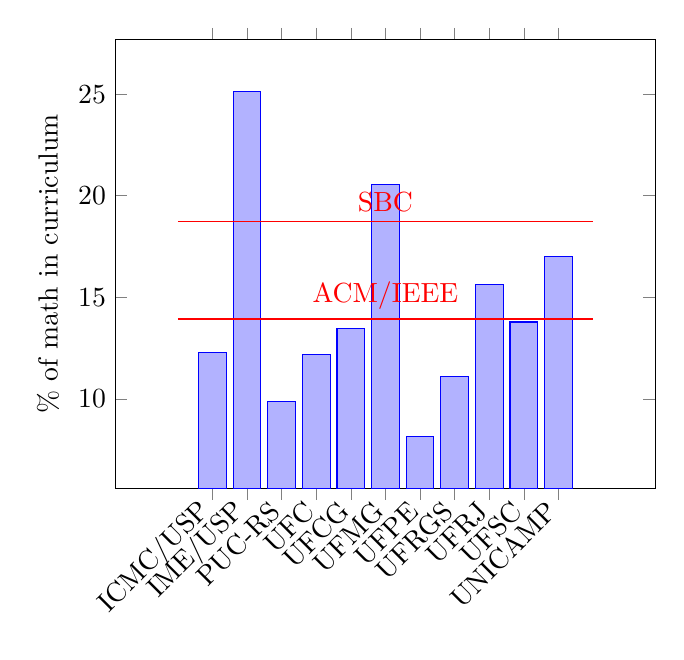
\begin{tikzpicture}
	\begin{axis}[
	ybar,
	enlargelimits=0.15,
	legend style={at={(0.5,-0.15)},
	anchor=north,legend columns=-1},
	ylabel={\% of math in curriculum},
	symbolic x coords={pre,ICMC/USP,IME/USP,PUC-RS,UFC,UFCG,UFMG,UFPE,UFRGS,UFRJ,UFSC,UNICAMP,pos},
	xtick=data,
%	nodes near coords,
%	nodes near coords align={vertical},
	x tick label style={rotate=45,anchor=east},
	]
	
	\addplot 
		coordinates {(ICMC/USP,12.29) (IME/USP,25.13) (PUC-RS,9.85) (UFC,12.20) (UFCG,13.46) (UFMG,20.57) (UFPE,8.15) (UFRGS,11.11) (UFRJ,15.61) (UFSC,13.78) (UNICAMP,17.00)};
	\addplot[red,sharp plot]
		coordinates {(pre,13.93) (pos,13.93)}
		node[above] at (axis cs:UFMG,13.93) {ACM/IEEE};
	\addplot[red,sharp plot]
		coordinates {(pre,18.75) (pos,18.75)}
		node[above] at (axis cs:UFMG,18.75) {SBC};
\end{axis}
\end{tikzpicture}
\caption{The proportion of mathematics in each curriculum compared with the reference curricula}
\end{figure}

	The most important fact derived from data is that few CS programs achieve the minimum hour load for math according to CS2008 or CR2005. This can be better visualized in Figure 1. Only IME/USP and UFMG fully meet the standards presented, while UFRJ and UNICAMP meet only CS2008. This implies that there is no evident correlation between the location of a CS program and its mathematical bias. Despite the fact that the ICMC/USP program is located near the math and statistics departments, it didn't achieve the minimum in both standards.
	

\section{Conclusions}
	In Brazil there are many undergraduate rankings available. Beyond Guia do Estudante, the ENADE ranking, for example, could be used to analyze a different set of universities. Just like Guia do Estudante, ENADE analyzes the infrastructure of the university and the level of professors' graduation, but also applies a test on a subset of the freshmen and senior students in order to evaluate the knowledge acquired in the graduation years. \cite{enade_info} Using the Preliminary Concept of Course (CPC) available at \cite{enade} the 10 best ranked universities are: Federal Universities of Rio Grande do Sul (UFRGS), Goiás (UFG), Campina Grande (UFCG), the city of Rio de Janeiro (Fluminense - UFF), Minas Gerais (UFMG), Pelotas (UFPel), Viçosa (UFV) and the Pampa (UNIPAMPA) and the private Universities of the West of São Paulo (UNOESTE) and of the North (UNINORTE). 
	
	With both comparisons another possibility is to analyze if there is a positive correlation between a highly ranked program in different rankings and the amount of mathematics studied during undergraduation. If so, further investigation may be necessary in order to find if there is a correlation of cause and effect between the math study and the quality of an undergraduate program.
	
	Finally, different studies are possible to measure the actual utility of a more theoretical topic in the professional life of a graduate. One possibility is to apply questionnaires to former students with the goal of identifying strengths and weaknesses of a curriculum.

% TODO Melhorar este parágrafo

	In this paper it was possible to see how mathematics disciplines are of great importance for a future graduate in Computer Science. It was presented that such subject is a base which needs to be robust to the development of more advanced topics which are based on it. Besides, many educators in the area of Computing with articles published in international events share that view.

	Moreover, it was noted that this area is experiencing a decline in its relevance, in part by the emergence of several new trends in the market that are absorbed in undergraduate curricula.
	
	Finally, an analysis of the current emphasis on mathematics in eleven Brazilian CS curricula from ten different universities was conducted through the study of absolute and relative workload in the area. It was found that only two programs fully and two other partially meet the minimum hour load for mathematics in an undergraduate CS curriculum according to two different academic standards, one national and the other international.
	
% An example of a floating figure using the graphicx package.
% Note that \label must occur AFTER (or within) \caption.
% For figures, \caption should occur after the \includegraphics.
% Note that IEEEtran v1.7 and later has special internal code that
% is designed to preserve the operation of \label within \caption
% even when the captionsoff option is in effect. However, because
% of issues like this, it may be the safest practice to put all your
% \label just after \caption rather than within \caption{}.
%
% Reminder: the "draftcls" or "draftclsnofoot", not "draft", class
% option should be used if it is desired that the figures are to be
% displayed while in draft mode.
%
%\begin{figure}[!t]
%\centering
%\includegraphics[width=2.5in]{myfigure}
% where an .eps filename suffix will be assumed under latex, 
% and a .pdf suffix will be assumed for pdflatex; or what has been declared
% via \DeclareGraphicsExtensions.
%\caption{Simulation Results}
%\label{fig_sim}
%\end{figure}

% Note that IEEE typically puts floats only at the top, even when this
% results in a large percentage of a column being occupied by floats.


% An example of a double column floating figure using two subfigures.
% (The subfig.sty package must be loaded for this to work.)
% The subfigure \label commands are set within each subfloat command, the
% \label for the overall figure must come after \caption.
% \hfil must be used as a separator to get equal spacing.
% The subfigure.sty package works much the same way, except \subfigure is
% used instead of \subfloat.
%
%\begin{figure*}[!t]
%\centerline{\subfloat[Case I]\includegraphics[width=2.5in]{subfigcase1}%
%\label{fig_first_case}}
%\hfil
%\subfloat[Case II]{\includegraphics[width=2.5in]{subfigcase2}%
%\label{fig_second_case}}}
%\caption{Simulation results}
%\label{fig_sim}
%\end{figure*}
%
% Note that often IEEE papers with subfigures do not employ subfigure
% captions (using the optional argument to \subfloat), but instead will
% reference/describe all of them (a), (b), etc., within the main caption.



% An example of a floating table. Note that, for IEEE style tables, the 
% \caption command should come BEFORE the table. Table text will default to
% \footnotesize as IEEE normally uses this smaller font for tables.
% The \label must come after \caption as always.
%
%\begin{table}[!t]
%% increase table row spacing, adjust to taste
%\renewcommand{\arraystretch}{1.3}
% if using array.sty, it might be a good idea to tweak the value of
% \extrarowheight as needed to properly center the text within the cells
%\caption{An Example of a Table}
%\label{table_example}
%\centering
%% Some packages, such as MDW tools, offer better commands for making tables
%% than the plain LaTeX2e tabular which is used here.
%\begin{tabular}{|c||c|}
%\hline
%One & Two\\
%\hline
%Three & Four\\
%\hline
%\end{tabular}
%\end{table}




% trigger a \newpage just before the given reference
% number - used to balance the columns on the last page
% adjust value as needed - may need to be readjusted if
% the document is modified later
%\IEEEtriggeratref{8}
% The "triggered" command can be changed if desired:
%\IEEEtriggercmd{\enlargethispage{-5in}}

\bibliographystyle{IEEEtran}
\bibliography{bibliography}


\end{document}


